\section{Anforderungen}
	\label{sec:requirements}
    
	\subsection{Eingabe}
    \label{sec:requirements-input}
 
    	Ziel dieser Arbeit ist die Entwicklung eines Prototypen einer Sprachapplikation. Mit dieser Applikation soll ein nichtsprechender und motorisch eingeschränkter Nutzer Sätze erzeugen können, die per Sprachausgabe ausgegeben werden können. Dabei soll es nicht nötig sein zu tippen. Sätze werden erzeugt, indem ein Wort nach dem anderen aus einer Liste von Wörtern ausgewählt wird. Am Ende wird der Satz bestätigt und ausgegeben. Sollte ein Wort ausversehen zum Satz hinzugefügt worden sein, muss es möglich sein, diesen Fehler zu korrigieren und das Wort wieder aus dem Satz zu entfernen. Das erste Wort in der Liste ist dabei das Wort, welches am wahrscheinlichsten als nächstes im aktuellen Satz vorkommen wird. Alle weiteren Wörter sind dann nach absteigender Wahrscheinlichkeit sortiert.
         
    	Dieses Kapitel befasst sich mit den Anforderungen bezüglich der Eingabe, die sich an die Applikation stellen. Wie im \autoref{sec:input-devices} beschrieben, sind die Eingabemethoden sehr verschieden. In vielen Fällen sind Eingabegerät und Software eng miteinander verbunden oder sogar ein in sich abgeschlossenes System.
        
        Um möglichst viele verschiedene Eingabegeräte zu unterstützen, soll die zu entwickelnde Applikation nicht direkt auf spezielle Geräte angepasst werden. Darum werden hier nicht bestimmte Aktionen zur Eingabe beschrieben, sondern Signale, welche dann von verschieden Geräten erzeugt werden können. Ein Signal kann jeder diskrete Code sein, der von einem Eingabegerät an die Software gesendet wird. Beispielsweise durch das Drücken einer bestimmten Taste auf einer Tastatur. Für die Entwicklung des Prototypen sollen Signale dann auch über die Tastatur erzeugt werden. 
        
        Da nicht jedes Eingabegerät die gleiche Anzahl an Signalen liefert, soll hier ein Minimum von drei diskreten Signalen festgelegt werden. Mit diesen drei Signalen sollen alle Funktionen der Applikation umzusetzen sein. Dabei ist es möglich, dass das gleiche Signal in einem anderen Kontext eine andere Bedeutung hat. Es ist auch vorstellbar, wenn unbedingt nötig, eine weitere Funktion durch Wiederholen des gleichen Signals innerhalb eines gewissen Zeitraums aufzurufen. 
        
        Diese Einschränkung wäre natürlich für Nutzer von Eingabegeräten, welche mehr als drei Signale erzeugen können, schnell frustrierend. So soll es möglich sein, auf weitere Signale zu reagieren und diese Erleichterungen bei der Bedienung der Applikation umzusetzen. Ein Beispiel hierfür wäre eine Liste, die sich über mehrere Zeilen erstreckt. Es ist möglich durch diese mit einem einzigen \emph{weiter} Befehl zu navigieren. Wenn möglich, wäre es aber auch wünschenswert, eine Zeile nach unten oder eben auch zurück zu navigieren.
        
        Bei der Betrachtung bestehender Eingabegeräte fallen weitere Anforderungen an die Bedienung der Applikation auf. Es gibt z. B. verschiedene Eingabegeräte für körperlich eingeschränkte Personen, die zur Steuerung eines Mauszeigers gedacht sind. Zum Beispiel die in \autoref{sec:input-devices} beschriebene Augensteuereng. Andere Geräte arbeiten, wie auch in \autoref{sec:input-devices} vorgestellt, mit verschieden angeordneten großen Tasten, manche bilden diese Tasten auch auf einem Touchscreen ab. Darum sollte es auch möglich sein, die Schaltflächen der Applikation klassisch per Maus oder Fingerdruck auswählen zu können. Dabei sollte auf die ungewöhnliche Steuerung des Mauszeigers und motorische Einschränkungen bei der Bedienung von Touchscreens Rücksicht genommen werden.
        
        Ziel dieser Abstrahierung der Eingabehandhabung ist der Versuch, die Grundlagen für ein modulares System zu skizzieren, welches auch mit zukünftigen noch nicht existierenden Eingabegeräten funktionieren kann.
        
	\subsection{Kategorieauswahl / -erkennung}
    \label{sec:requirements_categories}
    
    	Im folgenden soll der Ansatz einer manuellen Kategorienauswahl und einer nachfolgenden automatischen Kategorienerkennung beschrieben werden. Diese sollen in Kombination dazu beitragen, das Ergebnis der Prädiktion zu verbessern und somit die oben geforderte Bedienung ohne Tastatur möglich machen. Dabei wird auch in Kauf genommen, dass die Applikation eine bestimmte Art der Sprache und Wortwahl vorgibt. Dieser Ansatz bietet sich an, da die in \autoref{sec:software-examples} vorgestellte Software auch viel mit Kategorien arbeitet.
        
    	Da zur Prädiktion von wahrscheinlichen nächsten Wörtern zuerst einmal ein Satzanfang benötigt wird, startet man zu Beginn mit einer Kategorieübersicht. In dieser Übersicht sollen die Kategorien, wie sonst auch die Worte, als Liste dargestellt werden. Basierend auf der Kategorieauswahl wird dann eine Liste von möglichen ersten Wörtern eines Satzes angezeigt. 
        
        \begin{figure}[H]
    		\centering
    		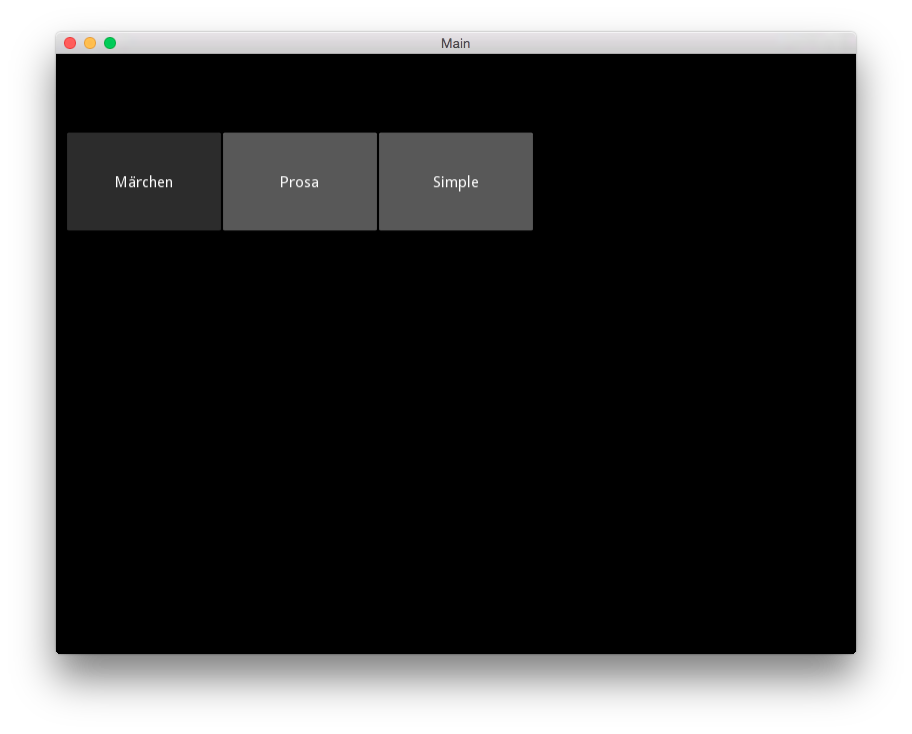
\includegraphics[width=.6\linewidth]{images/kategorien.png}
    		\caption[Aufbau der Grafischen Benutzeroberfläche]{Screenshot: Liste verfügbarer Kategorien}
    		\label{img:categories}
		\end{figure}
        
        Durch die enorme Einschränkung der möglichen Eingabesignale kann das Navigieren durch lange Listen sehr zeitaufwändig werden. Natürlich stehen im optimalen Fall die benötigten Wörter am Anfang der Liste. Es ist aber zu erwarten, dass es immer wieder Fälle gibt, bei denen keine sinnvolle oder hilfreiche Prädiktion gemacht werden kann. Um in diesen Fällen immer noch eine einigermaßen überschaubare und sinnvolle Liste erstellen zu können, soll der Wortschatz der Kategorie entsprechend eingeschränkt werden. Dabei ist es denkbar, mit Unterkategorien zu arbeiten, welche automatisch aufgrund der vorherigen Wörter bestimmt werden. Diese Unterkategorisierung soll im Hintergrund vom Nutzer unbemerkt stattfinden. 
        
        Oberkategorien dagegen werden vom Nutzer bewusst und manuell aus der in \autoref{img:categories} gezeigten Liste ausgewählt. Auch soll es zu jeder Zeit möglich sein, die bestehenden Oberkategorien zu wechseln, um somit Zugang zu einem anderen Vokabular zu erhalten.
        
        Eine Unterkategorie wird über eine Klassifizierung des letzten ausgewählten Wortes erkannt. Wie sehr sich Unterkategorien tatsächlich auf die Einschränkung oder doch nur auf die Sortierung des Ergebnisses auswirkt, soll im Verlauf der Implemetierung erprobt werden.
        
	\subsection{Ausgabe}
        
        Als letzter Teil der Anforderungen soll hier die visuelle Oberfläche der Applikation beschrieben werden. Diese richtet sich im Groben an der in \autoref{sec:software-examples} beschriebenen Software \emph{Tobii Sonar Scribe}. Da \emph{Tobii Sonar Scribe} allerdings wesentlich mehr Funktionen beinhaltet, soll die Oberfläche dieser Applikation sehr viel stärker reduziert werden. Der Hersteller \emph{Tobii} weist selbst in einem Anleitungsvideo auf die kleinen Schaltflächen der eigenen Applikation hin. \parencite[min. 0:53]{tobii:sonoScribeVideo} Diese Vereinfachung soll auch einer größeren Gruppe von Nutzern die Bedienung der Applikation ermöglichen.
        
        Die Applikation soll nicht für ein bestimmtes Endgerät oder eine bestimmte Bildschirmgröße entwickelt werden. Dennoch wird hier von einem Fenster, das ungefähr die Maße eines DIN A4 Blattes im Querformat aufweist, ausgegangen. Stark abweichende Bildschirmgrößen werden nicht berücksichtigt. Im oberen Teil des Bildschirms erstreckt sich vom linken bis zum rechten Rand eine Textzeile, in welcher der bisher generierte Satzteil angezeigt wird. Darunter befindet sich je nach Kontext die Liste der vorgeschlagenen Wörter oder Kategorien.
        
		\begin{figure}[H]
    		\centering
    		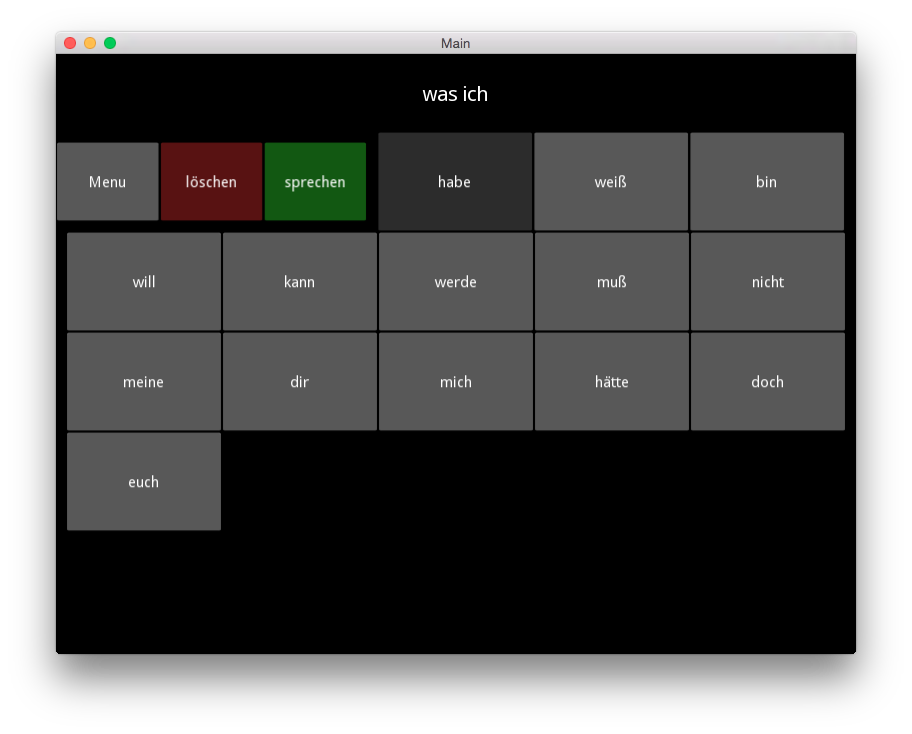
\includegraphics[width=.6\linewidth]{images/UI-Model.png}
    		\caption[Aufbau der Grafischen Benutzeroberfläche]{Screenshot: Aufbau der Grafischen Benutzeroberfläche}
    		\label{img:GUIBase}
		\end{figure}
        
        Sowohl die Liste der Wörter als auch die der Kategorien sollen als Raster von gleich großen Buttons dargestellt werden. Auf der ersten Position der Liste im Kontext der Wortvorschläge befindet sich ein Zurückknopf, mit welchem man zu der Kategorieübersicht gelangt. An zweiter Stelle ein Löschknopf. An dritter Stelle befindet sich ein Knopf zur Sprachausgabe. Das vorausgewählte Listenelement ist das vierte, so dass  man über das Zurücknavigieren in der Liste zuerst auf den Sprachknopf dann auf den Löschknopf und schließlich den Zurückknopf gelangt. Der bereits generierte Satz geht nicht verloren, wenn der Nutzer zurück zur Kategorieauswahl navigiert. Nach jedem ausgewählten Wort wird sofort die nächste Liste an vorgeschlagenen Wörtern generiert und angezeigt. Wenn ein Satz per Sprachausgabe gesprochen wird die Liste der bisher ausgewählten Wörter gelöscht.
	\newpage
